\clearpage
\hypertarget{conBran vis}{}
\subsection{Branching with statement nodes}
\visHeader

\begin{itemize}
  
\item[$\blacktriangleright$] Edit the \texttt{Box} class in your metamodel by invoking the \texttt{Operations} dialogue and creating a new method called
\texttt{initalizeBox}. Recalling the sole condition of conditional branching, set its return type to \texttt{EBoolean}. Save the method, then open the
\texttt{grow} SDM.

\item[$\blacktriangleright$] Add a new \texttt{StatementNode} named \texttt{initialize}. In the \texttt{Statement} tab, invoke a \texttt{MethodCallExpression}

\item[$\blacktriangleright$] Attach two \texttt{StopNode}s and appropriate edge guards to this new node. If the method call succeeds, the box could be
initialized, so return a literal \texttt{true}. If it failed however, \texttt{box} was already in an invalid state (by, e.g., having only one card) and we
return \texttt{false}. Overall, the new additions to \texttt{box.grow()} should resemble Fig.~\ref{fig:newGrowControl}.

\begin{figure}[htp]
\begin{center}
  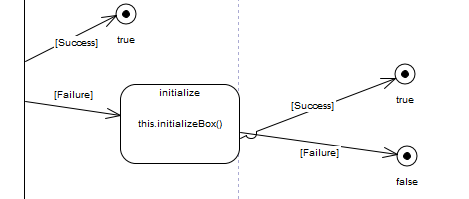
\includegraphics[width=0.8\textwidth]{ea_growControlAddition}
  \caption{The extended \texttt{grow} SDM \update}
  \label{fig:newGrowControl}
\end{center}
\end{figure}

\item[$\blacktriangleright$] Now that have edited our control flow, save, validate, and build your metamodel in Eclipse. Open \texttt{BoxImpl.java},
and navigate to \texttt{grow}, which starts at (approximately) line 207. Scan the comments until you find \texttt{//statement node `initialize'}.

\begin{figure}[htp]
\begin{center}
  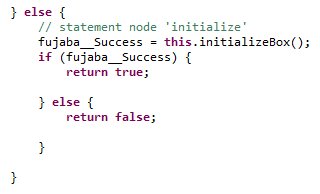
\includegraphics[width=0.5\textwidth]{eclipse_boxImplStatementNode}
  \caption{Code generated for branching with a statement node}
  \label{fig:initBoxImpl}
\end{center}
\end{figure}

\item[$\blacktriangleright$] Hold \texttt{ctrl} while clicking on the method to automatically jump to its declaration (Fig.~\ref{fig:initBoxDecl}).

\begin{figure}[htp]
\begin{center}
  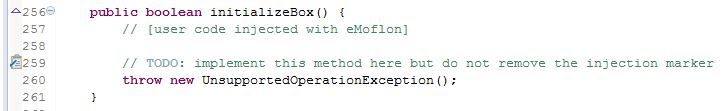
\includegraphics[width=\textwidth]{eclipse_initializeBoxDeclaration}
  \caption{The \texttt{initializeBox} declaration}
  \label{fig:initBoxDecl}
\end{center}
\end{figure}

\item[$\blacktriangleright$] You now have a choice -- you can either implement the method by hand here in Java as an injection, or you can return to
EA and implement it there as an SDM. The statement node will work just fine in both cases. Using Java makes sense if the method is non-structural, but
as we must check to see if there is a single partition, and then create the first two partitions of the box. This is actually quite structural and can be
described beautifully as a pattern.


 \item[$\blacktriangleright$] Switch back to your open \texttt{Box.grow} SDM in EA. You'll notice that if you double-click on \texttt{initialize}, the
 \texttt{Extract Story Pattern} option is invalid. This makes sense -- you don't define a pattern in a statement node. Instead, return to the main diagram and
 create a new SDM for \texttt{initializeBox}.
 
 \item[$\blacktriangleright$] Create a bounded \texttt{Box}, connected to a negative \texttt{onePartition}, and two partitions, \texttt{firstPartition} and
 \texttt{lastPartition}, both set to create. Also connect two true/false \texttt{StopNode}s. The pattern should now resemble Fig.~\ref{fig:buildPartitions}. The
 NAC is only fulfilled if the box has no partition, i.e., is in a pristine state and can be initialized.
 
 If grow is used for an empty box, it initializes the box the first time, then grows it after that, ensuring that the box is always in a valid state.
 
\item[$\blacktriangleright$] Save, validate, and build your metamodel. Review \texttt{BoxImpl.java} in the Eclipse workspace once again and take a look at the
generated implementation in \texttt{initializeBox}.
 
\newpage
 
 \vspace*{3cm}
 
 \begin{figure}[htp]
\begin{center}
  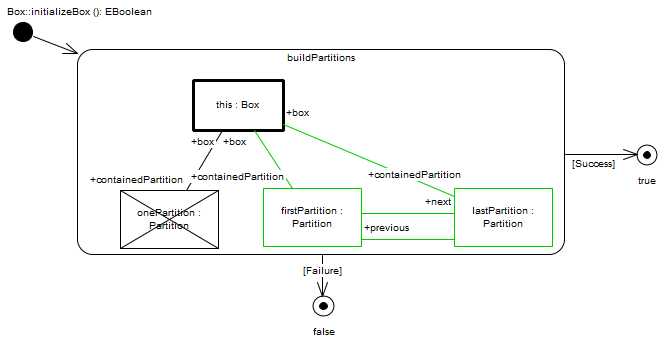
\includegraphics[width=\textwidth]{eclipse_buildPartitions}
  \caption{NAC to check for a single partition}
  \label{fig:buildPartitions}
\end{center}
\end{figure}

\jumpSingle{sec:extendedGui}

\end{itemize}
